% !TeX TS-program = xelatex
\documentclass[twoside=false,DIV=14]{scrartcl}

\usepackage{arev} % order matters, putting this above allows FiraSans to override it for body text
\usepackage[sfdefault]{FiraSans}
\usepackage{inconsolata}
%\usepackage[fira]{fontsetup}
\usepackage{scrlayer-scrpage}
\renewcommand{\titlepagestyle}{scrheadings}
\usepackage{graphicx}
\usepackage{blindtext}
\usepackage{wrapfig}
\usepackage{tabularx}
\usepackage{hyperref}
\usepackage{listings}
\usepackage{tikz}
\usepackage{amsmath}
\usepackage[many]{tcolorbox}

\usepackage{xcolor,sectsty}
\definecolor{blackish}{RGB}{56,58,54}
\definecolor{redish}{RGB}{109,41,49}
\definecolor{red}{RGB}{152,41,50}
\definecolor{orangeish}{RGB}{188,71,0}
\definecolor{blueish}{RGB}{25,33,139}
\subsubsectionfont{\color{blackish}}
\subsectionfont{\color{blackish}}
\sectionfont{\color{blackish}}

\lohead{\color{red} COMP3000 Programming Languages}
\rohead{
\includegraphics[width=0.5cm]{../logo.jpg}}

\setkomafont{author}{\sffamily \small}
\setkomafont{date}{\sffamily \small}

\DeclareOldFontCommand{\bf}{\normalfont\bfseries}{\mathbf}
\DeclareOldFontCommand{\tt}{\normalfont\ttfamily}{\texttt}

\lstset{basicstyle=\ttfamily}


\date{}
\newtcolorbox{aside}[1][]{
  title=Aside,
  width=0.3\textwidth,
  fonttitle=\bfseries,
  breakable,
  fonttitle=\bfseries\color{black},
  colframe=blueish!80,
  colback=blueish!2
  #1}

\newtcolorbox{note}[1][]{
  title=Note,
  width=\textwidth,
  fonttitle=\bfseries,
  breakable,
  fonttitle=\bfseries\color{black},
  colframe=orangeish!80,
  colback=orangeish!2
  #1}

\newtcolorbox{hint}[1][]{
    title=Hint,
    width=\textwidth,
    fonttitle=\bfseries,
    breakable,
    fonttitle=\bfseries\color{white},
    colframe=blueish!80,
    colback=blueish!2
    #1}

\newtcolorbox{todo}[1][]{
  title=!! TODO !!,
  width=\textwidth,
  fonttitle=\bfseries,
  breakable,
  fonttitle=\bfseries\color{white},
  colframe=red!80,
  colback=red!2
  #1}
  
\providecommand{\tightlist}{%
  \setlength{\itemsep}{0pt}\setlength{\parskip}{0pt}}


\title{\color{redish} \vspace{-2em}Week 6 Workshop: Binary Trees}

\begin{document}
{\color{blackish}\maketitle}\vspace{-2em}%\input{proposal.inc}
\begin{itemize}
    \item[$\cdot$] {\bf Resources:}  Week 5  Code Bundle.
    \item[$\cdot$] {\bf To submit this week's work:} Submit your solution to Exercise \ref{sec:submission} to your teacher in class.  Note, the exercises prior to \ref{sec:submission} will help you solve it, so try them first.  You should hand in a single piece of paper with your solution on it.  Be sure you include your name, student number, and the week number in the top-right of your submission.
\end{itemize}

\part*{Exercises}

\section{Binary Tree: Traversals}
Consider the following tree

% \usetikzlibrary{trees}
% \begin{tikzpicture}[level distance=1.5cm,
% level 1/.style={sibling distance=3cm},
% level 2/.style={sibling distance=1.5cm}]
% \node {a}
%   child {node {b}
%     child {node {d} child{node {h}}}
%     child {node {e} child{node {i}}}
%   }
%   child {node {c}
%     child {node {f}}
%     child {node {g} child{node {j}} child{node {k}}}
%   };
% \end{tikzpicture}

    
\begin{verbatim}
       a
     /   \
    b     c
   / \   / \
  d   e  f  g
 /   /     / \
h    i     j  k 
\end{verbatim}
            
For each of inorder, preorder and postorder traversals, state the order of the nodes printed. 

\section{Tree Traversal: Two from One}

If I give you only the \emph{pre-order} traversal for a tree, you can't uniquely determine the original tree\footnote{the same is true of the other orders}.  Draw \emph{two} possible trees that could generate the following pre-order traversal string
\begin{quote}
"nodnol"
\end{quote}
    
\section{Tree Traversal: Mystery Tree}
\label{sec:submission}

I've got a binary tree, but I'm keeping it secret.  I \emph{will} give you clues about it though.  These clues are enough for you to reconstruct the tree yourself.
\begin{itemize}
\item It is binary tree of \verb+char+s
\item The \emph{preorder} traversal is "myaeissmn"
\item The \emph{inorder} traversal is "easisymmn"
\item The \emph{post-order} traversal is "essiamynm"
\end{itemize}

Draw your guess at my original tree based on these clues.

\section{Tree Traversal: Is what?} 
What is the string that results from a \emph{breadth-first} traversal of the tree from question \ref{sec:submission}?

\section{Binary Tree Code: Add to Class}   
In your binary tree class, write functions for the following tasks.  Be sure to include tests for your functions.

\subsection{Balance}
 Returns the number of nodes on the right side minus the number of nodes on the left side.
\subsection{Max Element}
 Returns the largest value you can find in the tree.
\subsection{Generate Random Tree}
Write a \verb+static+ fucntion which generates random trees according to the following rules:
\begin{enumerate}
    \item The value is randomly chosen from 'a'-'z'.  This code might help
    \begin{lstlisting}
static Random r = new Random();
char c = (char)(r.nextInt(26) + 'a');
    \end{lstlisting}
    \item There is a 30\% chance there is a left child.
    \item There is a 30\% chance there is a right child.
\end{enumerate}
Write a main method which can test out how your generation method works.  What happens if the chance of a child goes over 50\%?

\subsection{Iterative?}
Try writing an iterative version of \emph{max elements}.  What do you notice?

\newpage\setcounter{section}{0}
\part*{Solutions}

\section{Binary Tree: Traversals}
\begin{description}
    \item[pre-order] "abdheicfgjk"
    \item[in-order] "hdbieafejgk"
    \item[post-order] "hdiebfjkgca"   
\end{description}

\section{Tree Traversal: Two from One}

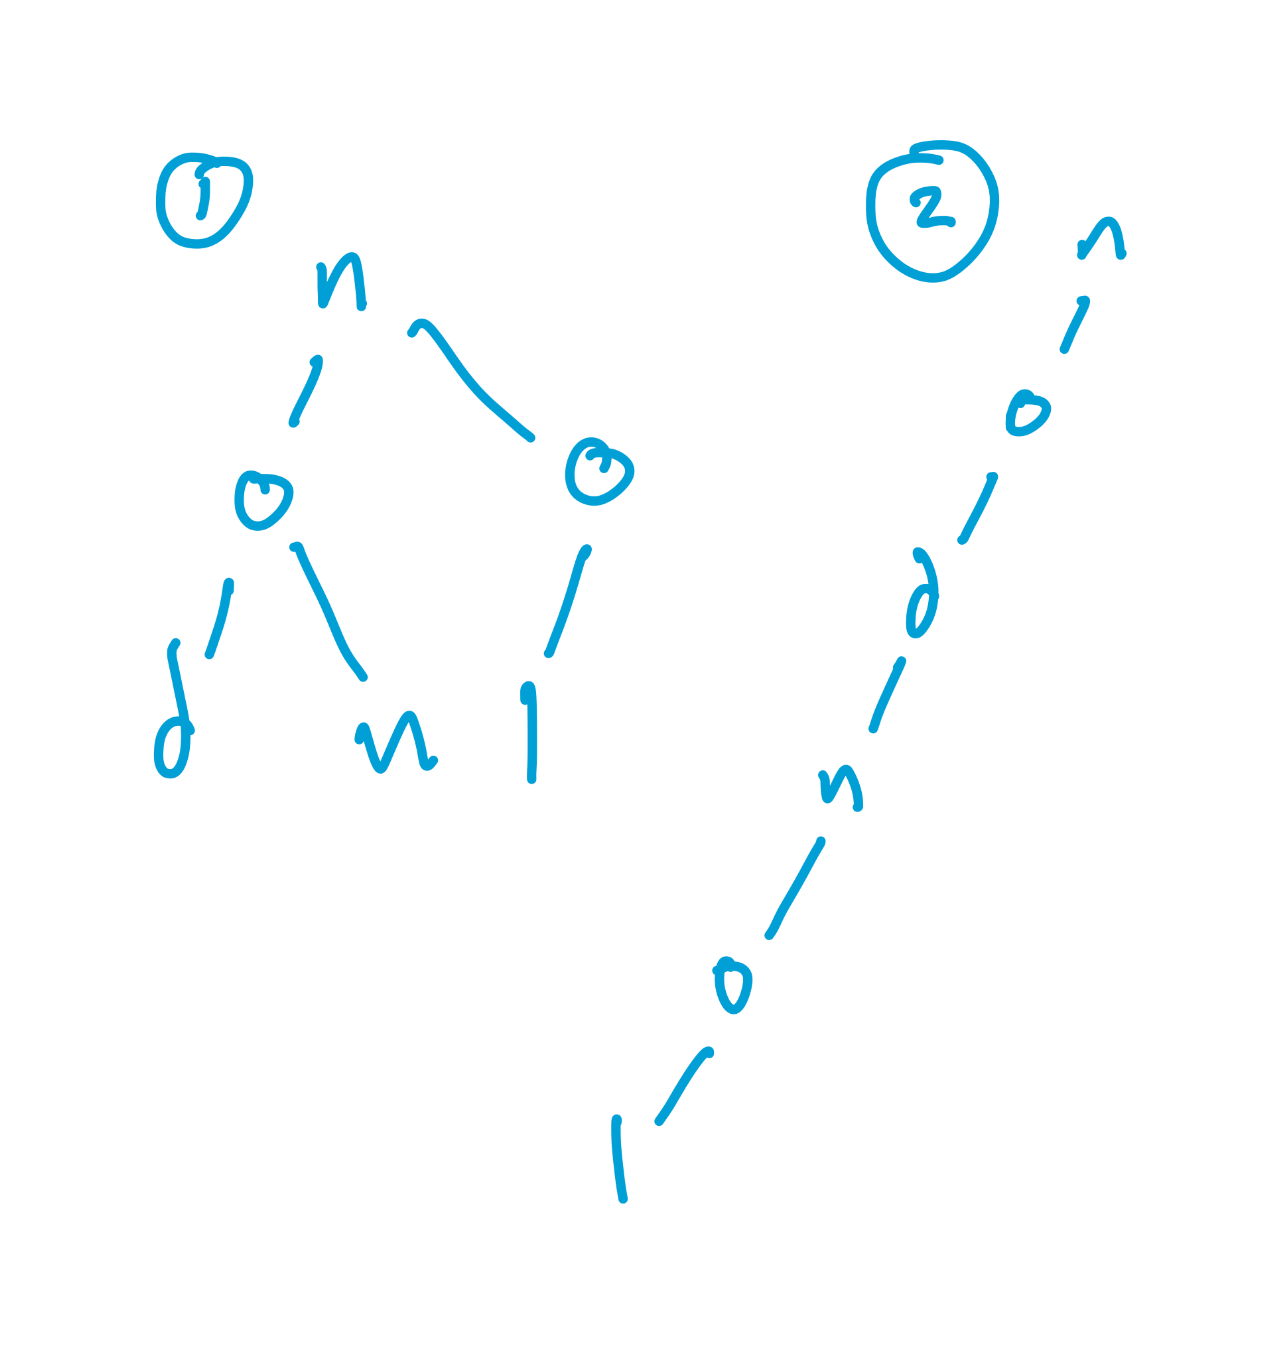
\includegraphics[width=0.7\textwidth]{nodnol.jpeg}
\section{Tree Traversal: Mystery}

\begin{note}
It is \emph{theoretically possible} to construct multiple different trees which match a traversal set.  Thus there \emph{could} be other solutions besides this one.  However, I have not been able to find them and thus I think this is one of those cases where the three traversals are enough to \emph{uniquely} determine the tree.
\end{note}

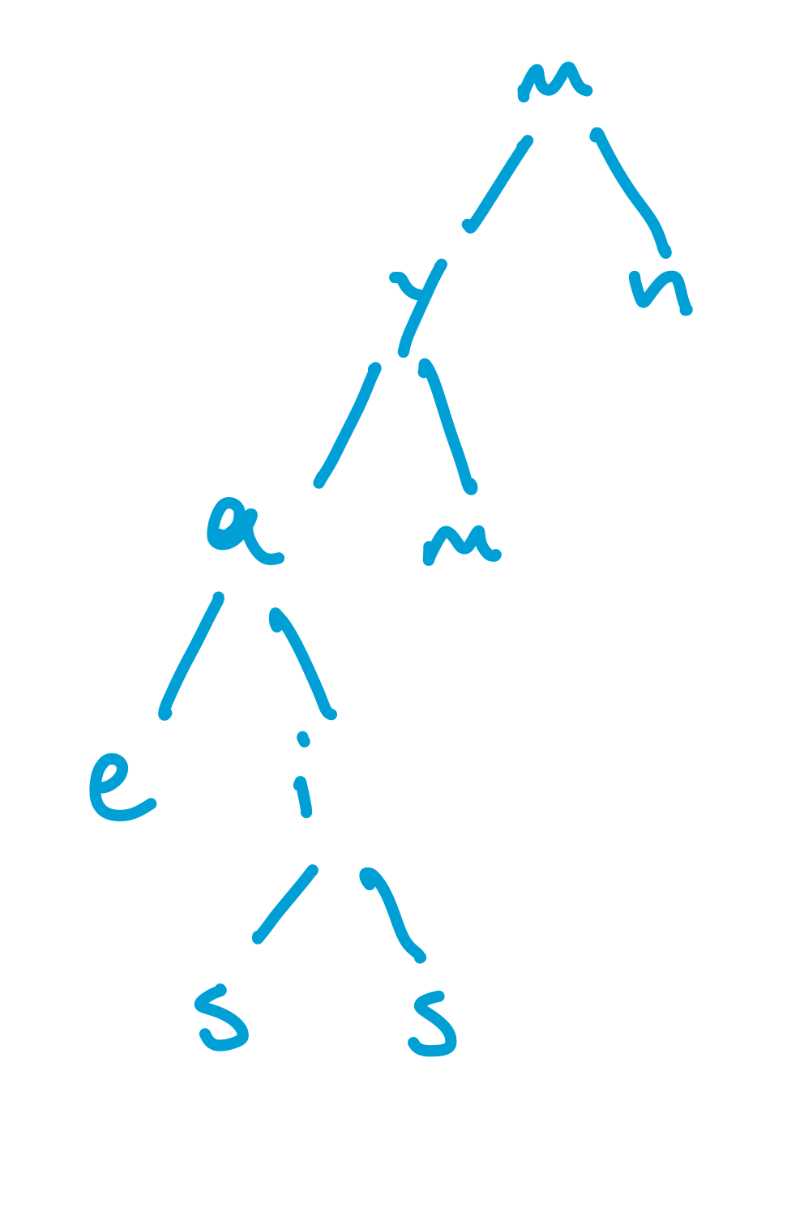
\includegraphics[width=0.5\textwidth]{mystery_tree_one.jpeg}

\section{Tree Traversal: Is what?}

"mynameiss"

\section{Binary Tree Code: Add to Class}
\subsection{Balance}
\begin{lstlisting}[language=java]
int balance(){
    int left  = (this.left == null)? 0: this.left.size();
    int right = (this.right == null)? 0: this.right.size();
    return left - right;
}

@Test
public void testBalance(){
    BinaryTree ex = BinaryTree.exampleTree();
    assertEquals(ex.balance(), 1);
    assertEquals(ex.invert().balance(), -1);
    ex.addAt('z', "lll");
    assertEquals(ex.balance(), 2);
    assertEquals(ex.invert().balance(), -2);

}
\end{lstlisting}

\subsection{Max Element}
I do a cool trick here.  I know the max element must be at least \verb+value+ so I use that value in the places that I have null pointers as the "fallback" value.  I found that Java was lacking an easy way to get the max of two characters, so I added a private method to do that.  It made my code much easier to read overall.
\begin{lstlisting}
private char max_of_char(char a, char b){
    if (a > b) return a;
    return b;
}
char max(){
    char left = (this.left == null)? value: this.left.max();
    char right = (this.right == null)? value: this.right.max();
    return max_of_char(value, max_of_char(left, right));
}
@Test
public void testMax(){
    BinaryTree ex = BinaryTree.exampleTree();
    assertEquals(ex.max(), 'f');
    assertEquals(ex.invert().max(), 'f');
    ex.addAt('z', "llrlrlrllrl");
    assertEquals(ex.max(), 'z');
}    
\end{lstlisting}

\subsection{Generate Random Tree}
My main method prints out a frequency distribution for tree sizes.  They mostly end up quite small.
\begin{lstlisting}
public static BinaryTree generateRandom(int prob){
    char c = (char)(r.nextInt(26) + 'a');
    BinaryTree left = (r.nextInt(100) < prob)? generateRandom(prob): null;
    BinaryTree right = (r.nextInt(100) < prob)?generateRandom(prob): null;
    return new BinaryTree(c,left,right);
}
public static void main(String[] args){
    int[] buckets = new int[10000];
    for(int i = 0; i < 100; i++){
        buckets[generateRandom(30).size()]++;
    }
    for(int i = 0; i < 10; i++){
        System.out.println(String.valueOf(i) + "," + String.valueOf(buckets[i]));
    }
}
\end{lstlisting}

If you attempt to adjust the probability to make them longer, you can succeed to some extent but there is a point at which the maximum likely length blows up massivly and the computer will stack overflow.  This tends to happen at about 50\% probability.

One trick to generate larger trees is to diminish the probability of children as the depth of the tree increases.

\subsection{Iterative}
My attempts failed.  The challenge is that there are \emph{two} recursive calls.  A loop just does the same thing over and over.  It can't easily \emph{double} each time.  While it was relatively easy to make loop versions of \emph{single} recursion, it is harder to write loop versions of \emph{double} recursion.

Another angle to think about is the time complexity.  Traversing a binary tree is $O(2^n)$ in the depth of the tree, what type of loops will run that many times?

It is possible of course, but you end up \emph{linearising} the tree on the way so it is likely to cause more confusion if I go into it too deeply.  Let's leave it at "its much harder!".

\newpage\setcounter{section}{0}
\part*{Self Study}

\section{Binary Tree Code: Add a node to an existing tree}
If you are asked to add a node to the end of a linked list, you know exactly where it goes.  If I ask you to do the same for a binary tree you should ask "which end?".  A binary tree has more than one free end slot you could choose.

Add an \verb+addAt+ method to your \verb+BinaryTree+ class which takes two parameters:
\begin{enumerate}
\item the \verb+char+ to add
\item a \verb+String+ describing \emph{how to find the free spot we are interested in}.  The description is given as a series of "l" and "r" values telling you which branch to take in search of a free slot.  As soon as a free slot is encountered, you add the value there.  If the string runs out of letters, do nothing.  It is not a problem if there are letters remaining in the string when you find a free slot.
\end{enumerate}

\subsection{Recursive version}
Write a recursive version of this method.

\subsection{Iterative version}
Write an iterative version of this method.

Compare your efforts to what you found working on the \emph{max elements} function.  Why was this effort so much easier?

\section{Binary Tree: Ternary Tree}
In this question we will extend a binary tree into a \emph{Ternary tree}.  Such a tree has \emph{three} children instead of two.  We will label them "left", "middle", and "right".
\subsection{Draw}
Draw a diagram of a Ternary tree storing strings.  You can put whatever you like in the tree.

\subsection{Code}
Create a new class \verb|TernaryTree|, which you have copied from the \verb|BinaryTree| class, and make the necessary adjustments to make it work.  Don't try to rewrite all the methods, they don't all make sense, but \emph{do} write:
\begin{enumerate}
\item The constructor(s)
\item size
\item depth
\item preorder traversal
\end{enumerate}

\subsection{Other Orders}
Only one of \emph{in-order} and \emph{post-order} can be written for ternary trees.  Which and why?

\newpage\setcounter{section}{0}
\part*{Self Study Solutions}

\section{Binary Tree Code: Add a node to an existing Binary Tree}
I think this is the first time you get to see my binary tree testing trick.  Testing the output of tree methods gets very tedious if I have to construct the tree I am expecting as the output.  Instead, I use the combination of pre and post-order traversal outputs to check against.  This is not 100\% fool-proof but it is good enough for my purposes and lets me test many more cases for the same amount of effort, so I think it is a win overall.

\subsection{Recursive Version}

\begin{lstlisting}[language=java]
void addAt(char newval, String path){
    if (path.length() == 0)
        return;
    if (path.charAt(0) == 'l'){
        if(left == null){
            left = new BinaryTree(newval, null, null);
        } else {
            left.addAt(newval, path.substring(1));
        }
    }
    if (path.charAt(0) == 'r'){
        if(right == null){
            right = new BinaryTree(newval, null, null);
        } else {
            right.addAt(newval, path.substring(1));
        }
    }
    return;
}

@Test
public void testAddAt(){
    BinaryTree rootA = new BinaryTree('a', null, null);
    assertEquals(rootA.preorder(), "a");
    rootA.addAt('b', "l");
    assertEquals(rootA.preorder(), "ab");
    rootA.addAt('c', "r");
    assertEquals(rootA.preorder(), "abc");
    assertEquals(rootA.postorder(), "bca");
    rootA.addAt('d', "ll");
    assertEquals(rootA.preorder(), "abdc");
    assertEquals(rootA.postorder(), "dbca");
    rootA.addAt('e', "lrl");
    assertEquals(rootA.preorder(), "abdec");
    assertEquals(rootA.postorder(), "debca");
    rootA.addAt('f', "lrl");
    assertEquals(rootA.preorder(), "abdefc");
    assertEquals(rootA.postorder(), "dfebca");
}

\end{lstlisting}

\subsection{Iterative Version}
I had the \emph{worst} time writing this iterative version. I had a bug that took me ages to find.  The problem was that I was using \verb+left+ and \verb+right+ in places I should have been using \verb+curr.left+ and \verb+curr.right+. It reminded me of the hidden cost of having to keep references to similar things in a function and reminded me that, even if they seem harder to understand, recursive versions are better!

\begin{lstlisting}[language=java]
void addAtIterative(char newval, String path){
    BinaryTree curr = this;
    int atLoc = 0;
    while (path.length() > atLoc && curr != null){
        char direction = path.charAt(atLoc);
        if (direction == 'l'){
            if (curr.left == null){
                curr.left = new BinaryTree(newval, null, null);
                break;
            } else {
                curr = curr.left;
                atLoc++;
            }
        } else {
            if (curr.right == null){
                curr.right = new BinaryTree(newval, null, null);
                break;
            } else {
                curr = curr.right;
                atLoc++;
            }
        }
    }
}

@Test
public void testAddAtIterative(){
    BinaryTree rootA = new BinaryTree('a', null, null);
    assertEquals(rootA.preorder(), "a");
    rootA.addAtIterative('b', "l");
    assertEquals(rootA.preorder(), "ab");
    rootA.addAtIterative('c', "r");
    assertEquals(rootA.preorder(), "abc");
    assertEquals(rootA.postorder(), "bca");
    rootA.addAtIterative('d', "ll");
    assertEquals(rootA.preorder(), "abdc");
    assertEquals(rootA.postorder(), "dbca");
    rootA.addAtIterative('e', "lrl");
    assertEquals(rootA.preorder(), "abdec");
    assertEquals(rootA.postorder(), "debca");
    rootA.addAtIterative('f', "lrl");
    assertEquals(rootA.preorder(), "abdefc");
    assertEquals(rootA.postorder(), "dfebca");
}

\end{lstlisting}
I was able to write an iterative version because \emph{it doesn't try to traverse the whole tree}.  The function only needs to explore one path in the tree, which is just like a linked list.  We are ignoring a branch each time so we don't come up against the problem that we had with max elements.

\section{Binary Tree: Ternary Tree}
\subsection{Draw}
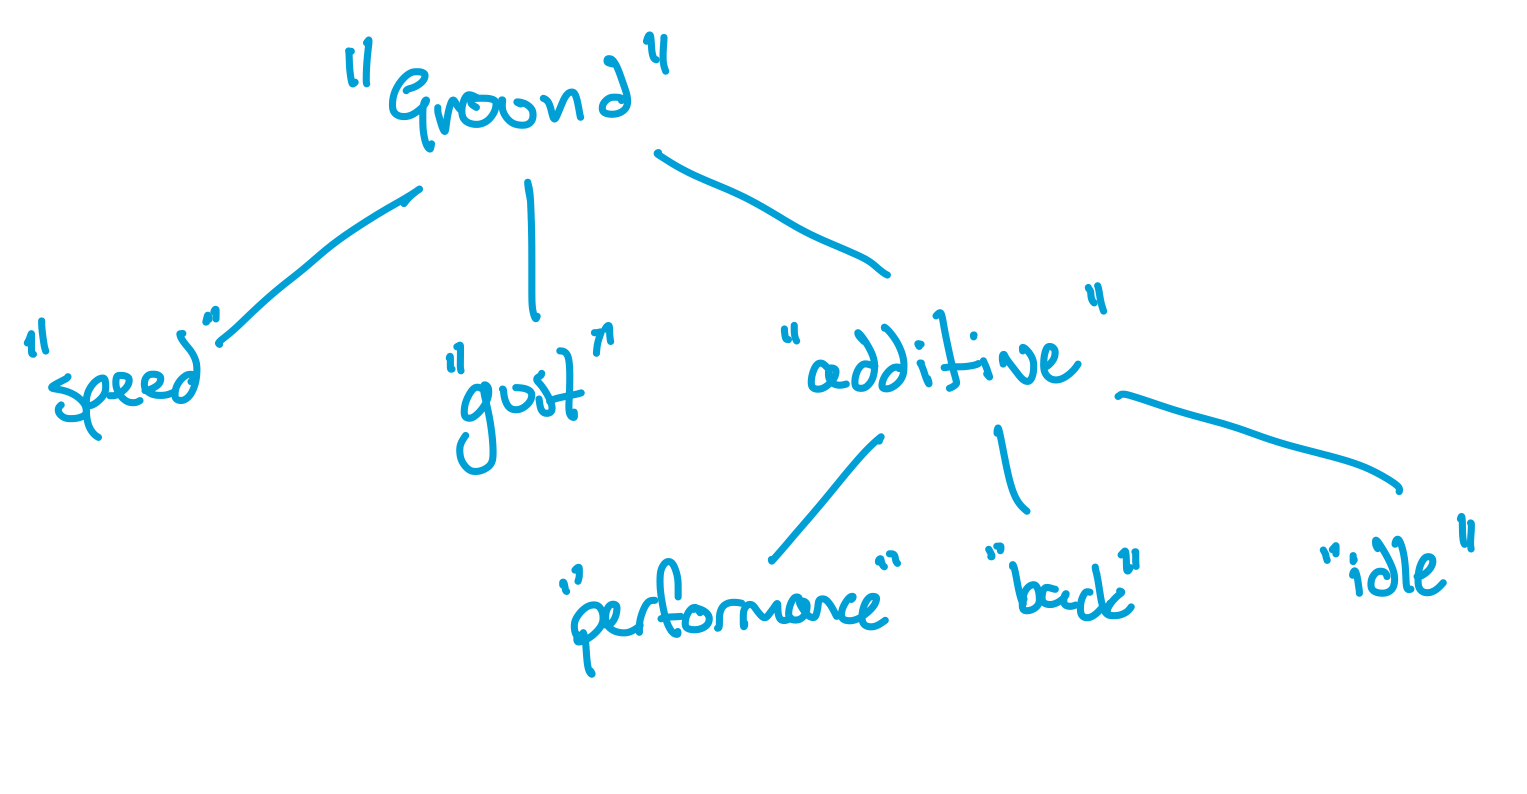
\includegraphics[width=0.8\textwidth]{ternary_tree.jpeg}

\subsection{Code}
Here is my solution.  I chose to call the various children \verb+left+, \verb+middle+, \verb+right+ which seems the obvious choice.  Everything was standard.  I am very glad to have the expression form of \verb+if+ because the code could have just spread out way too much if I didn't.\footnote{Thanks to the blancolirio channel for providing example strings when my imagination had run dry}
{\scriptsize
\begin{lstlisting}[language=java]
import org.junit.Test;
import static org.junit.Assert.assertEquals;

public class TernaryTree {
    TernaryTree left;
    TernaryTree middle;
    TernaryTree right;
    String value;

    public TernaryTree(){}

    TernaryTree(String value, TernaryTree left, TernaryTree middle, TernaryTree right){
        this.value = value;
        this.left = left;
        this.middle = middle;
        this.right = right;
    }
    int size(){
        int l = (left == null)? 0: left.size();
        int m = (middle == null)? 0: middle.size();
        int r = (right == null)? 0: right.size();
        return 1 + l + m + r;
    }

    int depth(){
        int l = (left == null)? 0: left.depth();
        int m = (middle == null)? 0: middle.depth();
        int r = (right == null)? 0: right.depth();
        return 1 + Math.max(l, Math.max(m,r));
    }

    String preorder(){
        String l = (left == null)? "": left.preorder();
        String m = (middle == null)? "": middle.preorder();
        String r = (right == null)? "": right.preorder();
        return value + l + m + r;
    }

    @Test
    public void basicTests(){
        TernaryTree ex = new TernaryTree("Ground",
                                            new TernaryTree("speed", null, null, null),
                                            new TernaryTree("gust", null, null, null),
                                            new TernaryTree("additive", 
                                                            new TernaryTree("performance", null, null, null),
                                                            new TernaryTree("back", null, null, null),
                                                            new TernaryTree("idle", null, null, null)
                                                            )
                                            );
        assertEquals(ex.size(), 7);
        assertEquals(ex.depth(), 3);
        assertEquals(ex.preorder(), "Groundspeedgustadditiveperformancebackidle");
    }
    
}     
\end{lstlisting}
\subsection{Other Orders}
Only post-order makes sense.  In-order means that the value is emitted after the left node is visited and before the right node is visited.  In a ternary tree, we would need to decide if it happens before or after the middle node is visited.  There are really \emph{two different} in-order traversals possible and we would have to arbitrarily choose one.  Arbitrary decisions are bad news in programming.

\end{document}